\documentclass[10pt]{beamer}
\usepackage[latin1]{inputenc}
\usetheme{Warsaw}
\usecolortheme{orchid}
\usepackage{color}
%\usepackage{braket}
\usepackage{amsmath}
\usepackage{amsfonts}
\usepackage{amssymb}
\usepackage{graphicx}
%\setbeamerfont{page number in head/foot}{size=\normalsize}
%\setbeamertemplate{footline}[frame number]
\usepackage{ifthen}
\usepackage{animate}
\usepackage{movie15}
\usepackage{xmpmulti}

\newcommand*\oldmacro{}%
\let\oldmacro\insertshorttitle%
\renewcommand*\insertshorttitle{%
	\oldmacro\hfill%
	\insertframenumber\,/\,\inserttotalframenumber}
\setbeamercovered{invisible}
\usepackage{tikz}
\usetikzlibrary{calc}
\usepackage{pgfplots}
\usepackage{tikz-3dplot}
\usetikzlibrary{decorations.markings}
\usetikzlibrary{shapes,arrows}
\newcommand{\midarrowright}{\tikz \draw[-triangle 90] (0,0) -- +(.1,0);}
\newcommand{\midarrowup}{\tikz \draw[-triangle 90] (0,0) -- +(0,.1);}

\usetikzlibrary{shadings, calc, decorations.markings}
\tikzset{->-/.style={decoration={
			markings,
			mark=at position #1 with {\arrow{<}}},postaction={decorate}},
	->-/.default=0.3,
}

\tikzset{->>-/.style={decoration={
			markings,
			mark=at position #1 with {\arrow{<}}},postaction={decorate}},
	->>-/.default=0.7,
}

%\theoremstyle{definition}
%\newtheorem{definition}{Definition}

\theoremstyle{plain}
\newtheorem{prop}{Proposition}

\newcommand\ds{\displaystyle}
\newcommand\ts{\textstyle}
\newcommand{\mb}{\mathbf}
%\renewcommand{\thenotation}{}
%\renewcommand{\theequation}{\thesection.\arabic{equation}}
\def\Caption #1{\caption{\footnotesize #1}}
%\renewcommand\Caption{#1}{\Caption{\small{#1}}}
%\def\Caption #1{\Caption{\small{{#1}}}}

\def \Bfemph #1{\textbf{\emph{#1}}}


%\def\Proof.{{\medbreak\noindent{\it Dimostrazione}\enspace}}
\def\Proof{{\medbreak\noindent{\textbf{Proof.} }}}
\def\Proofsketch{{\medbreak\noindent{\textbf{Sketch of proof.} }}}
\def\endproof{~\hfill $\blacksquare$}
%\def\endproof{\hfill$\square$\par\medskip}

\def\Svolgimento{{\medbreak\noindent{\textit{Execution.} }}}
\def\Suggerimento{{\medbreak\noindent{\textit{Hint:} }}}


\def\mR{{\mathbb R}}
\def\mC{{\mathbb C}}
\newcommand{\parz}[2]{ \frac{\partial #1}{\partial #2}}
\newcommand{\deri}[2]{\displaystyle \frac{\dd #1}{\dd #2}}
\renewcommand{\Re}{\text{Re }}
\renewcommand{\Im}{\text{Im }}
%\renewcommand{\theta}{\vartheta}
\newcommand{\Int}{\text{Int }}
\newcommand{\Ext}{\text{Ext }}
\newcommand{\supp}{\text{supp}}
\newcommand{\mD}{\mathcal{D}}
\newcommand{\dd}{\mathrm d}
\newcommand{\norm}[1]{\displaystyle \left \| #1 \right \|}
\renewcommand{\div}{\operatorname{div}}
\newcommand{\rot}{\operatorname{rot}}
\newcommand{\grad}{\operatorname{grad}}
\newcommand{\id}{\mathds{1}}
\newcommand{\mM}{\mathrm{M}}
\newcommand{\mT}{\mathrm{T}}
%\renewcommand{\to}{\longrightarrow}
\newcommand{\scalar}[2]{\left\langle #1, #2 \right\rangle}
\newcommand{\mf}[1]{\mathbf{#1}}

\def\Xint#1{\mathchoice 
	{\XXint\displaystyle\textstyle{#1}}% 
	{\XXint\textstyle\scriptstyle{#1}}% 
	{\XXint\scriptstyle\scriptscriptstyle{#1}}% 
	{\XXint\scriptscriptstyle\scriptscriptstyle{#1}}% 
	\!\int} 
\def\XXint#1#2#3{{\setbox0=\hbox{$#1{#2#3}{\int}$} 
		\vcenter{\hbox{$#2#3$}}\kern-.5\wd0}} 
\def\Mint{\Xint -}


\renewcommand{\hat}[1]{\widehat{#1}}
\renewcommand{\theta}{\vartheta}
\renewcommand{\epsilon}{\varepsilon}
%\renewcommand{\phi}{\varphi}
\newcommand{\res}{\mathop{\mathrm{Res }}}

\newcommand{\colonna}[2]{\begin{pmatrix}
		#1 \\ #2
\end{pmatrix}}
\newcommand{\riga}[2]{\begin{pmatrix}
		#1 & #2
\end{pmatrix}}
%%%%%%%%%%%%%%%%%%%%%%%%%%%%%%%%%%%%%%%%%%%%%%%%%%%%%%%%%%%%%%%%%%%%%%%%%%%%%%%%%%%%%%%%%%%

\newcounter{angle}
\setcounter{angle}{0}

\title{Introduction to Quantum Backflow}
\author{Eugenio Mauri}
\date

\begin{document}
	\begin{frame}
		%\begin{figure}
		%	\centering
		%	
\includegraphics{../unipv}
		%\end{figure}
		\maketitle
		\footnotesize Supervisor: Prof. Claudio Dappiaggi\\
		Co-supervisor: Dot. Nicol� Drago
	\end{frame}
	%\begin{frame}
	%	\frametitle{Guideline}
	%	\tableofcontents
	%\end{frame}
	
	\section{Introduction}
	%\begin{frame}
	%	\frametitle{What Quantum Backflow is?}
	%	\begin{itemize}
	%		\item<+-> \alert{Backflow} is a quantum "counter-intuitive" effect (such as tunneling, uncertainty relations, ...).
	%		\item<+-> It consists on particles with momentum pointing \alert{"right-wards"}, but whose probability density flows \alert{"left-wards"}.
	%	\end{itemize}
	%\end{frame}
	\begin{frame}
		\frametitle{What Quantum Backflow is?}
		\textbf{Setting}: Consider a non-relativistic \alert<1>{free particle} in one dimension\pause
		\begin{itemize}
			\item Suppose that at time $t=0$ the particle has \alert<2>{positive momentum} with probability $1$.\pause
			\item Consider the probability $P(t)$ of finding the particle in $x<0$ at time $t$. What is the \alert<3>{time-dependence} of $P(t)$?
		\end{itemize}\pause
		Answers:
		\begin{itemize}
			\item[] In \alert{classical physics}: $P(t)$ is always decreasing with time.\pause
			\item[] In \alert{quantum physics}: not necessarily.
		\end{itemize}
	\end{frame}
	
	\begin{frame}
				\frametitle{What Quantum Backflow is?}
		\multiinclude[format=png, start=1,graphics={scale=0.5}]{../images/gand}
	\end{frame}
	
	\begin{frame}
				\frametitle{What Quantum Backflow is?}
		\centering
		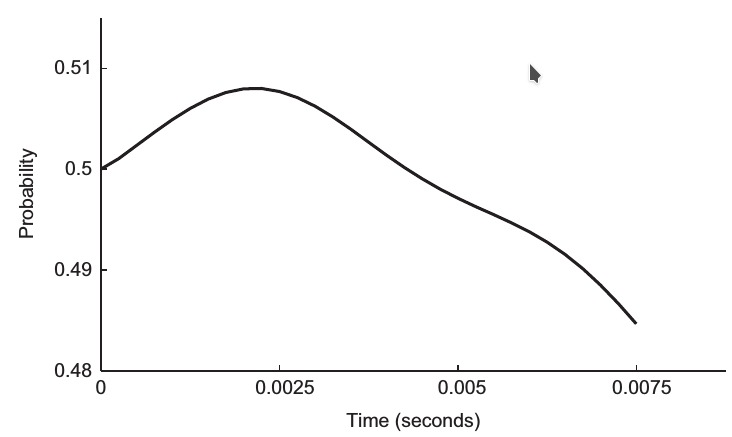
\includegraphics[scale=0.4]{../images/P(T)}
	\end{frame}
	
	
	\section{Backflow in Free Theory}
	\begin{frame}
		\frametitle{Right-movers}
		What does it means that a particle "travels to the right"?\pause
		\begin{definition}
			Let $\psi\in L^2(\mR)$ be a wave-function for a single particle.  We call $\psi$ a \alert<2>{\textbf{right-mover}} if $\mathrm{supp}\ \hat{\psi}\in[0,+\infty)$.
		\end{definition}\pause
		\begin{definition}
			We call $E_\pm:L^2(\mR)\to L^2(\mR)$ the operator such that:
			\begin{equation*}
			\mathcal{F}[E_\pm\psi](p)=\theta(\pm p)\hat{\psi}(p)\ \forall \psi\in L^2(\mR),
			\end{equation*}
			where $\theta$ is the Heaviside function.
		\end{definition}
	\end{frame}
	
	%\begin{frame}
	%	\frametitle{Temporal boundedness of backflow}
	%		Given a right-mover $\psi=E_+\psi$, \alert{backflow} occurs whenever the density probability current function $j_\psi=-i/2[\psi^*\partial_x\psi-\psi\partial_x\psi^*]$ assumes \alert{negative values}.
	%\pause
	%	\begin{block}{Question:}
	%		What is the \alert{maximum amount} of probability which could flow back
	%		through a point $x_0$ during an interval of time $T$ for a \alert{right-moving}
	%		free-particle?
	%	\end{block}
	%\end{frame}
	
	\begin{frame}
		\frametitle{Temporal boundedness of backflow}
		\begin{itemize}
			\item[-]<1-> Probability as a quadratic form
			\begin{equation*}
			L(\psi_T):=\int_{0}^{+\infty}\!\!\!|\psi_T(x)|^2\, \dd x=(\hat{\psi}|\underbrace{\widehat{U}^*_T\mathcal{F}\theta\mathcal{F}^{-1} \widehat{U}_T}_{:=\tilde{\theta}_T}\hat{\psi})\ \text{with}\ \widehat{U}_T=\mathcal{F}U_T\mathcal{F}^{-1}.
			\end{equation*}
			\item[-]<2-> Flux in $[-T,T]$: $(\hat{\psi}|(\tilde{\theta}_{-T}-\tilde{\theta}_T)\hat{\psi})=(\hat{\psi}|B_T\hat{\psi})$.
			\item[-]<3-> $B_T$ is called \alert<3>{\textbf{backflow operator}}, and it is \alert<3>{bounded} and \alert<3>{self-adjoint}.
			\item[-]<4->\alert<4>{\textbf{Backflow constant}}: $\lambda:=\sup\{(\phi|\theta B_T \theta \phi)\ |\ \|\phi\|=1,\ T>0 \}$
		\end{itemize}
	\end{frame}
	
	\begin{frame}
		\frametitle{Temporal boundedness of backflow}
	    \begin{itemize}
	    	\item[-] Equivalently, \alert<1>{$\lambda=\sup\bigcup_{T>0}\sigma(\theta B_T\theta)$}\pause
	    	\item[-] Scaling arguments show $\sigma(\theta B_{T_1}\theta)=\sigma(\theta B_{T_2}\theta)$ for all $T_1,T_2>0$. Hence \alert<2>{$\lambda=\sup \sigma(\theta B_{T=1}\theta)$}.\pause
	    \end{itemize}
		\begin{theorem}[\textbf{Temporal boundedness of backflow}]
			Let $\lambda=\sup \sigma(\theta B\theta)$, where $B=B_{T=1}$ is the backflow operator. For any right-mover $\psi\in L^2(\mR)$ such that $\psi=E_+\psi$ and for any $T>0$ it holds 
			\begin{equation*}
			\int_{0}^{T}\!\!\!\!j_\psi(0,t)\, \dd t\ge -\lambda>-\infty.
			\end{equation*}
		\end{theorem}\pause
		\Proof $\sigma( \theta B\theta) \subseteq [-\|B\|,\|B\|]$ since the operator $\theta B\theta$ is bounded and self-adjoint.\endproof
	\end{frame}
	
	\begin{frame}
		\frametitle{Maximum backflow approximation}
		\begin{prop}
			Let $K:L^2(\mR_+)\to L^2(\mR_+)$ be the integral operator:
			\begin{equation*}
			\label{eq:bracken_int}
			(Kf)(u)=-\frac{1}{\pi}\int_{0}^{\infty}\frac{\sin(u^2-v^2)}{u-v}f(v)\, \dd v \ \ \forall f\in L^2(\mR_+).
			\end{equation*}
			Then $\theta B\theta f  = Kf$ for all $f\in L^2(\mR_+)$.
		\end{prop}\pause
		\textbf{Ingredients:} Hilbert transform \begin{equation*}
		(Hf)(p)=\frac{1}{\pi}PV\!\!\!\int_{-\infty}^{\infty}\frac{f(q)}{p-q}\, \dd q.
		\end{equation*}
		
	We can use $K$ to \alert{approximate} $\lambda$.
	\end{frame}
	
	\begin{frame}
		\begin{figure}[h]	
			\centering
			\begin{minipage}{0.45\textwidth}
				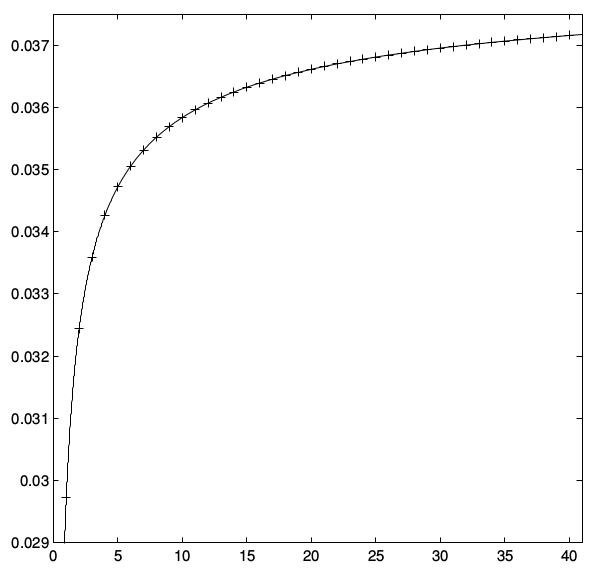
\includegraphics[scale=0.25]{../images/backflow_approx_1}
				%\caption{$\lambda$ plotted against $h$ and fit $\lambda_\infty+b/\sqrt h$.}
				%\label{fig:backflow_approx_1}
			\end{minipage}
			\hfil
			\begin{minipage}{0.45\textwidth}
				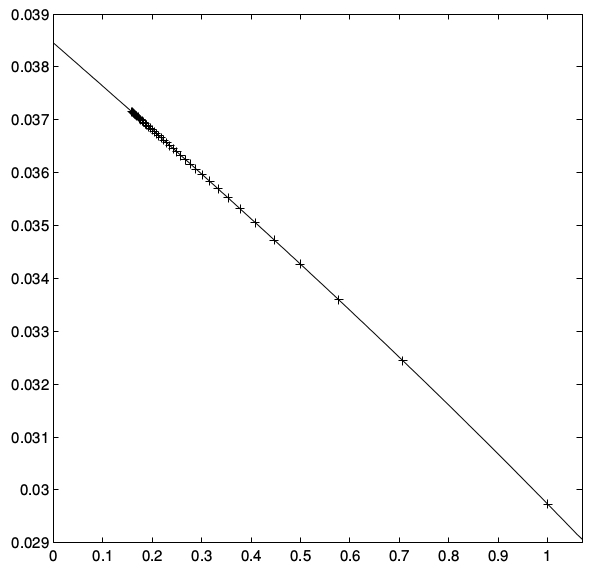
\includegraphics[scale=0.25]{../images/backflow_approx_2}
				%\caption{$\lambda$ plotted against $1/\sqrt h$ and polynomial fit of third order.}
				%\label{fig:backflow_approx_2}
			\end{minipage}
		\end{figure}
		\begin{center}
		\Large $\lambda\approx0.0384517$
		\end{center} 
	\end{frame}
	
	\begin{frame}
		\frametitle{Spatial extension of Backflow}
		What about the spatial properties of backflow?\pause 
		\begin{itemize}
			\item[-] Current as a quadratic form (not an operator) $j_\psi(x)\equiv(\psi|J(x)\psi)$.\pause
			\item[-] The average, for test functions $f$, $\int_{\mR}f(x)j_\psi(x)\,\dd x\equiv (\psi|J(f)\psi)$ exists as operator.\pause
 		\end{itemize}
 		\begin{block}{Lemma}
 			The quadratic form $E_+J(x)E_+$ is unbounded from above and from below.
 		\end{block}
 		\textbf{NB}: Unboundedness from below as superposition of high and low momentum.\pause
 		\begin{prop}
 			For any $f\in \mathcal{S}(\mR)$, $f\ge0$, there exists a constant $\beta_0(f)\in(f)\in(-\infty,0)$ such that $(\psi|E_+J(f)E_+\psi)\ge\beta_0(f)$.
 		\end{prop}
	\end{frame}
	
	\section{Backflow in Scattering Theory}
	\begin{frame}
		\frametitle{Asymptotic right-movers}
		Take an \alert<1>{interacting} system with the Hamiltonian $H=H_0+V$.\pause
		\begin{itemize}
			\item[-] Time evolution $e^{iHt}$ \alert<2>{does not preserve} the space of right-movers $E_+(L^2(\mR))$.\pause
			\item[-] \alert<3>{Reflection} may destroy backflow.\pause
		\end{itemize}
		Consider states \textit{incoming} \alert<4-5>{right-moving asymptotics} and \alert<4-5>{M\o{}ller operator}:\pause
		\begin{equation*}
			\Omega_V:=\lim_{t\to-\infty}e^{itH}e^{-itH_0}
		\end{equation*}\pause
		\begin{itemize}
			\item[-] exists under regularity and short-range assumptions on $V$.\pause
			\item[-] links "free" solutions of Schr\"{o}dinger equation with "interacting" solutions.
		\end{itemize}
	\end{frame}
	
	\begin{frame}
		\frametitle{Asymptotic right-movers}
		\begin{definition}
			Let $V\in L^1(\mR)$ be a potential. We referred to $V$ as a "short-range"  potential (indicated $V\in L^{1+}(\mR)$) if it satisfies $\|V\|_{1+}=\int_{\mR}\!\dd x\,(1+|x|)|V(x)|<+\infty$.
		\end{definition}\pause
		\begin{theorem}
			Let $V\in L^{1+}(\mR)$. Then
			\begin{itemize}
				\item[(a)] $\Omega_V$ exists.
				\item[(b)] $[-\partial_x^2+2V(x)-k^2]\psi(x)=0$ has unique solutions
				\begin{equation*}
					\varphi_k(x)=\begin{cases}
					T_V(k)e^{ikx}+o(1) & \text{for }  x\to+\infty\\
					e^{ikx}+R_V(k)e^{-ikx}+o(1) & \text{for } x\to-\infty
					\end{cases}
				\end{equation*}
				\item[(c)] For any $\hat{\psi}\in C_0^\infty(\mR)$, $(\Omega_VE_+\psi)(x)=\frac{1}{\sqrt{2\pi}}\int_{0}^{\infty}\!\varphi_k(x)\hat{\psi}(k)\, \dd k.$
			\end{itemize}
		\end{theorem}
	\end{frame}
	
	\begin{frame}
		\frametitle{Backflow and Scattering}
		We search bounds for the \alert{averaged current}, $f\ge0$\pause
		\begin{equation*}
			\int_{\mR}f(x)j_{\Omega_VE_+\psi}(x)\, \dd x=(\psi|E_+\Omega_V^*J(f)\Omega_VE_+\psi).
		\end{equation*}\pause
		Expanding $E_+\Omega_V^*J(f)\Omega_VE_+$ we have
		\begin{equation*}
			(\psi|E_+\Omega_V^*J(f)\Omega_VE_+\psi)\ge \beta_0(f)-2\alert<4>{\|J(f)(i+P)^{-1}\|}[2+\alert<5>{\|P(\Omega_V-T_V)E_+\|}].
		\end{equation*}\pause
		\begin{itemize}
			\item[-] we have $\alert<4>{\|J(f)(i+P)^{-1}\|}\le\|f\|_{\infty}+\frac{1}{2}\|f'\|_{\infty}$.\pause
			\item[-] We need to evaluate $\alert<5>{\|P(\Omega_V-T_V)E_+\|}$.
		\end{itemize}
	\end{frame}
	
	\begin{frame}
		\frametitle{Backflow and Scattering}
		\begin{block}{Lemma}
			Let $V\in L^{1+}(\mR)$. Then, there exists $c_V\in\mR$ such that
			\begin{equation*}
				\|P(\Omega_V-T_V)E_+\|\le 2c_V\|V\|_{1+}
			\end{equation*}
		\end{block}\pause
		\Proofsketch Rewrite the time-independent Schr\"{o}dinger equation as (Lippman-Schwinger equation)
		\begin{equation*}
				\varphi_k(x)=T_V(k)e^{ikx}+\int_{-\infty}^{\infty}\! 2V(y)G_k(y-x)\varphi_k(y)\, \dd y,
		\end{equation*}
		where $G_k(x)=\sin(kx)\theta(x)/k$\pause, and estimate 
		\begin{equation*}
			(P(\Omega_V-T_V)E_+\psi)(x)=\frac{-i}{\sqrt{2\pi}}\frac{\dd}{\dd x}\int_{0}^{\infty}\!\!\!\!\!\dd k\int_\mR\!\! \dd y\, V(y)G_k(x-y)\varphi_k(y)\tilde{\psi}(k)
		\end{equation*}
		with the known asymptotics for $\varphi_k(x)$
	\end{frame}
	
	\begin{frame}
		\frametitle{Backflow and Scattering}
		\begin{theorem}[\textbf{Boundedness of Backflow in scattering scenarios}]
			For any potential $V\in L^{1+}(\mR)$ and for any non-negative $f\in\mathcal{S}(\mR)$, there exists a constant $\beta_V(f)\in(-\infty,0)$ such that
			\begin{equation*}
			(\psi|E_+\Omega_V^*J(f)\Omega_VE_+\psi)\ge\beta_V(f)\ \forall\ \psi\in L^2(\mR).
			\end{equation*}
		\end{theorem}\pause
		\begin{itemize}
			\item[-] Reflection processes \alert<2>{do not destroy} boundedness of backflow.\pause
			\item[-] Heuristic explanation: Backflow is a \alert<3>{high momentum effect}, but for high momentum reflection component is \alert<3>{suppressed}.\pause
			\item[-] What about \alert<4>{experimental} observations? (Bose-Einstein condensate, Bragg pulse, superposition of different momentum sates...)
		\end{itemize}
	\end{frame}
	
	\begin{frame}
		\frametitle{Experimental set-up}
		\begin{figure}
			\centering
			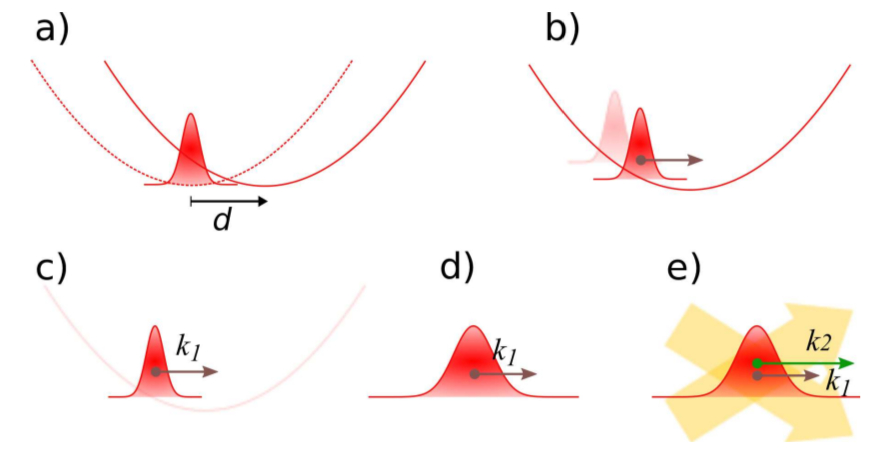
\includegraphics[scale=0.3]{../images/bose}
		\end{figure}
		
	\end{frame}
	
	\begin{frame}
		\begin{center}
			\huge Thank you for your attention!
		\end{center} 
	\end{frame}
	
\end{document}
